\subsection{Overall Architecture}
\subsubsection{Overall}
The Raspberry Pi Model 4B collects data from three devices--imaging sensor, GPS, and a current clamp. 
The imaging sensor counts the number of people inside the PRT car, the GPS hat tracks the current location of the PRT car, and the current clamp monitors the voltage and current being drawn by the PRT car. 
These three devices transfer their data to the Raspberry Pi. 
Once the Pi is stopped for about 5 seconds and has a Wi-Fi connection to WVU Encrypted, the data transfers to a SQL database hosted on a Google Cloud server instance. 
Next, a web application retrieves the data from the SQL database to visualize it, providing graphs and charts to analyze relationships between the data. 
The overall architecture is in Figure 2 and Figure 3, which represents the system functionality from top to bottom.

\begin{center}
    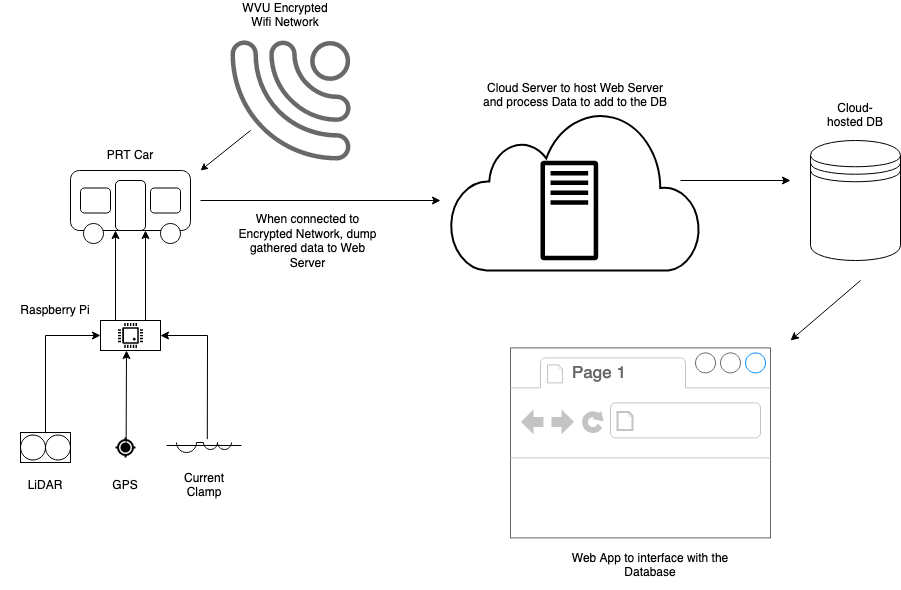
\includegraphics[width=0.5\textwidth]{Overall_Architecture.png}\\
    Fig 2. Overall Architecture
\end{center}

\begin{center}
    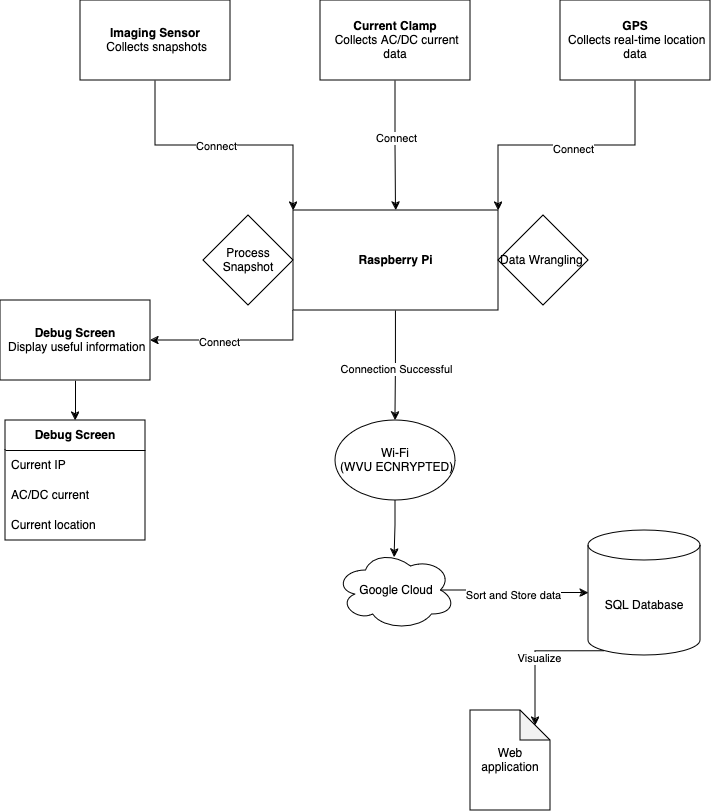
\includegraphics[width=0.5\textwidth]{System_Functionality.png}\\
    Fig 3. System Functionality
\end{center}

\subsubsection{Hardware}
Four devices fit onto the Raspberry Pi for the collection of data. 
The connections are shown below in Figure 4. 
The Pi communicates with the GPS for real-time location. 
The antenna plugs into the GPS and realizes the data collection. 
The current clamp collects AC voltage and current readings, recording it to the Pi.
A debug screen displays the GPS status, IP address, and the current AC reading for debugging purposes. 
The debug screen configures the subsystem, ensuring that the components work. 
Lastly, the imaging sensor collects snapshots of people for detecting the number of people in a PRT car. 
The snapshots go to the Raspberry Pi, where the Pi will use an algorithm to count the number of people in that snapshot.

\begin{center}
    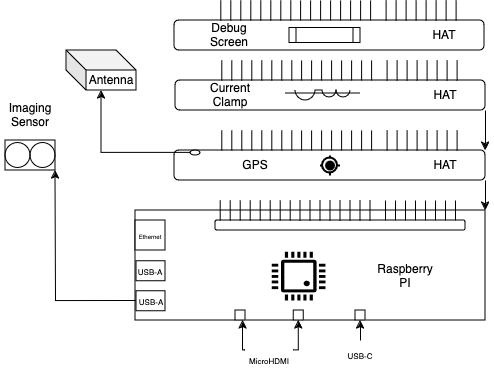
\includegraphics[width=0.5\textwidth]{Hardware_Architecture.png}\\
    Fig 4. Hardware Architecture
\end{center}

\subsubsection{Software}
When the Raspberry Pi obtains a Wi-Fi connection through WVU Encrypted and is at a standstill for 5 seconds or more, data goes to Google Cloud. 
Figure 5 represents the process of data transfer once Wi-Fi connects. 
The Google Cloud hosts a SQL database that sorts and stores all the metadata from the Pi system. 
A web application uses this sorted data from the SQL database, providing visualization through charts and graphs to highlight relationships in the data. 
The web application provides opportunities for identifying potential risks in the system, such as irregular AC current or voltage on a specific PRT car.

\begin{center}
    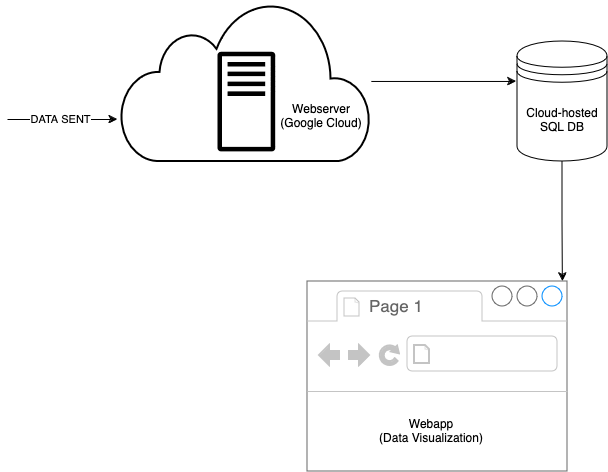
\includegraphics[width=0.5\textwidth]{Software_Architecture.png}\\
    Fig 5. Software Architecture
\end{center}

\subsection{System Design}
\subsection{Overall Architecture}
\subsubsection{Overall}
The Raspberry Pi Model 4B collects data from three devices--imaging sensor, GPS, and a current clamp. 
The imaging sensor counts the number of people inside the PRT car, the GPS hat tracks the current location of the PRT car, and the current clamp monitors the voltage and current being drawn by the PRT car. 
These three devices transfer their data to the Raspberry Pi. 
Once the Pi is stopped for about 5 seconds and has a Wi-Fi connection to WVU Encrypted, the data transfers to a SQL database hosted on a Google Cloud server instance. 
Next, a web application retrieves the data from the SQL database to visualize it, providing graphs and charts to analyze relationships between the data. 
The overall architecture is in Figure 2 and Figure 3, which represents the system functionality from top to bottom.

\begin{center}
    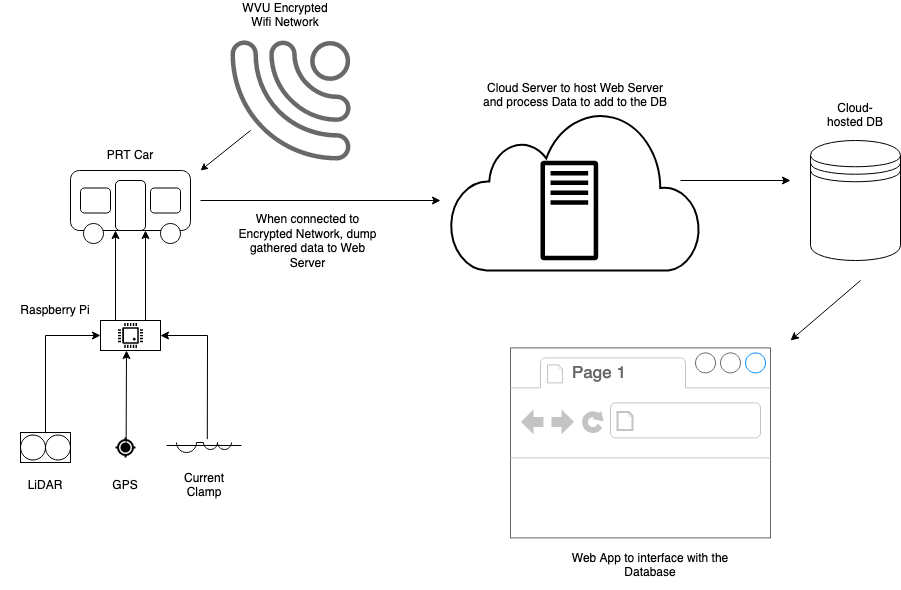
\includegraphics[width=0.5\textwidth]{Overall_Architecture.png}\\
    Fig 2. Overall Architecture
\end{center}

\begin{center}
    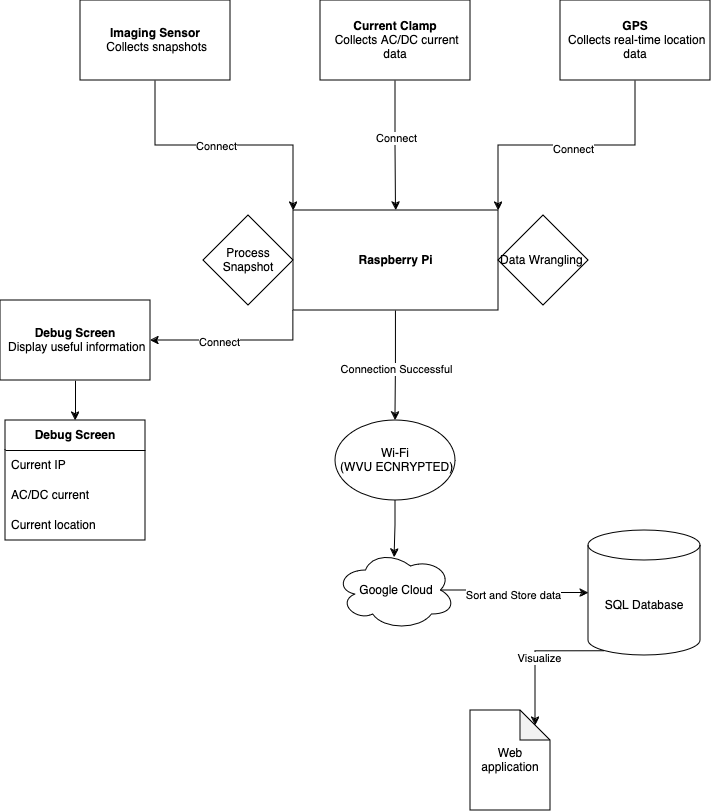
\includegraphics[width=0.5\textwidth]{System_Functionality.png}\\
    Fig 3. System Functionality
\end{center}

\subsubsection{Hardware}
Four devices fit onto the Raspberry Pi for the collection of data. 
The connections are shown below in Figure 4. 
The Pi communicates with the GPS for real-time location. 
The antenna plugs into the GPS and realizes the data collection. 
The current clamp collects AC voltage and current readings, recording it to the Pi.
A debug screen displays the GPS status, IP address, and the current AC reading for debugging purposes. 
The debug screen configures the subsystem, ensuring that the components work. 
Lastly, the imaging sensor collects snapshots of people for detecting the number of people in a PRT car. 
The snapshots go to the Raspberry Pi, where the Pi will use an algorithm to count the number of people in that snapshot.

\begin{center}
    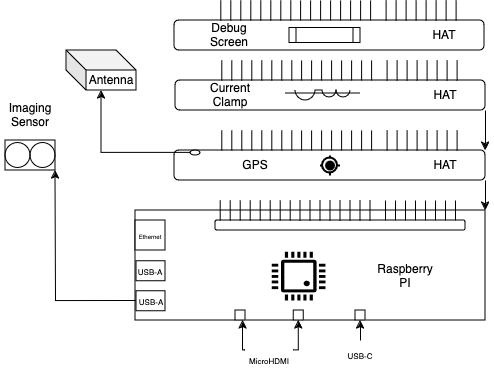
\includegraphics[width=0.5\textwidth]{Hardware_Architecture.png}\\
    Fig 4. Hardware Architecture
\end{center}

\subsubsection{Software}
When the Raspberry Pi obtains a Wi-Fi connection through WVU Encrypted and is at a standstill for 5 seconds or more, data goes to Google Cloud. 
Figure 5 represents the process of data transfer once Wi-Fi connects. 
The Google Cloud hosts a SQL database that sorts and stores all the metadata from the Pi system. 
A web application uses this sorted data from the SQL database, providing visualization through charts and graphs to highlight relationships in the data. 
The web application provides opportunities for identifying potential risks in the system, such as irregular AC current or voltage on a specific PRT car.

\begin{center}
    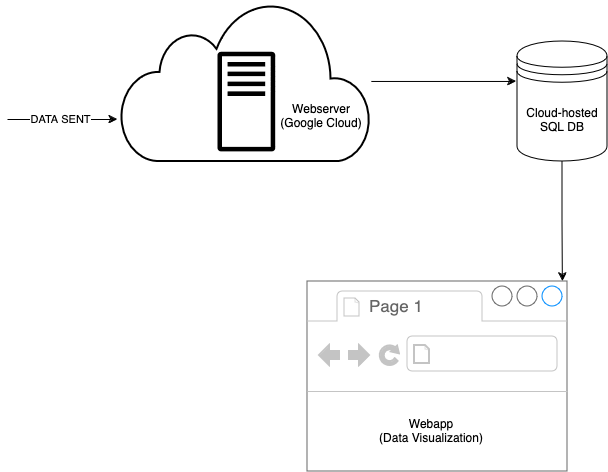
\includegraphics[width=0.5\textwidth]{Software_Architecture.png}\\
    Fig 5. Software Architecture
\end{center}

\subsection{System Design}
\subsection{Overall Architecture}
\subsubsection{Overall}
The Raspberry Pi Model 4B collects data from three devices--imaging sensor, GPS, and a current clamp. 
The imaging sensor counts the number of people inside the PRT car, the GPS hat tracks the current location of the PRT car, and the current clamp monitors the voltage and current being drawn by the PRT car. 
These three devices transfer their data to the Raspberry Pi. 
Once the Pi is stopped for about 5 seconds and has a Wi-Fi connection to WVU Encrypted, the data transfers to a SQL database hosted on a Google Cloud server instance. 
Next, a web application retrieves the data from the SQL database to visualize it, providing graphs and charts to analyze relationships between the data. 
The overall architecture is in Figure 2 and Figure 3, which represents the system functionality from top to bottom.

\begin{center}
    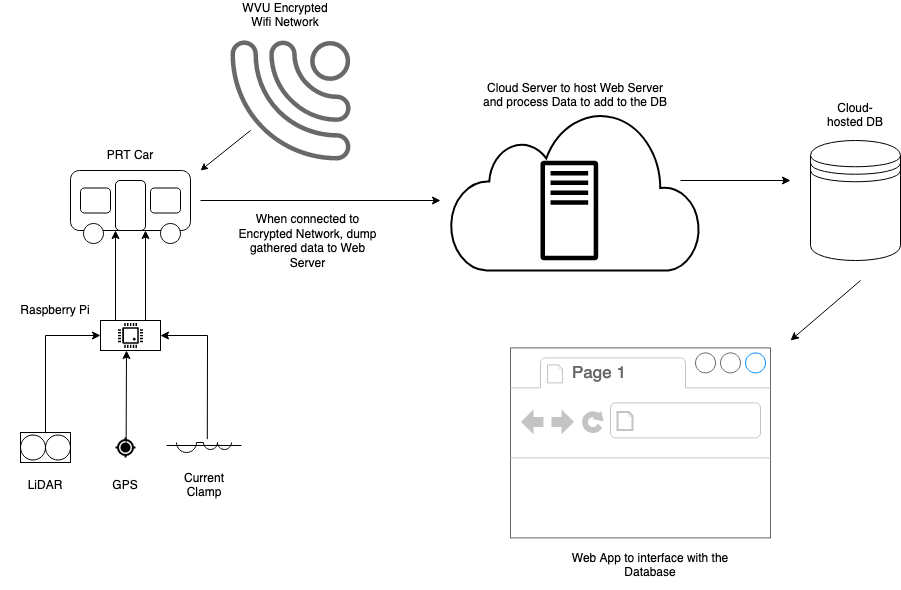
\includegraphics[width=0.5\textwidth]{Overall_Architecture.png}\\
    Fig 2. Overall Architecture
\end{center}

\begin{center}
    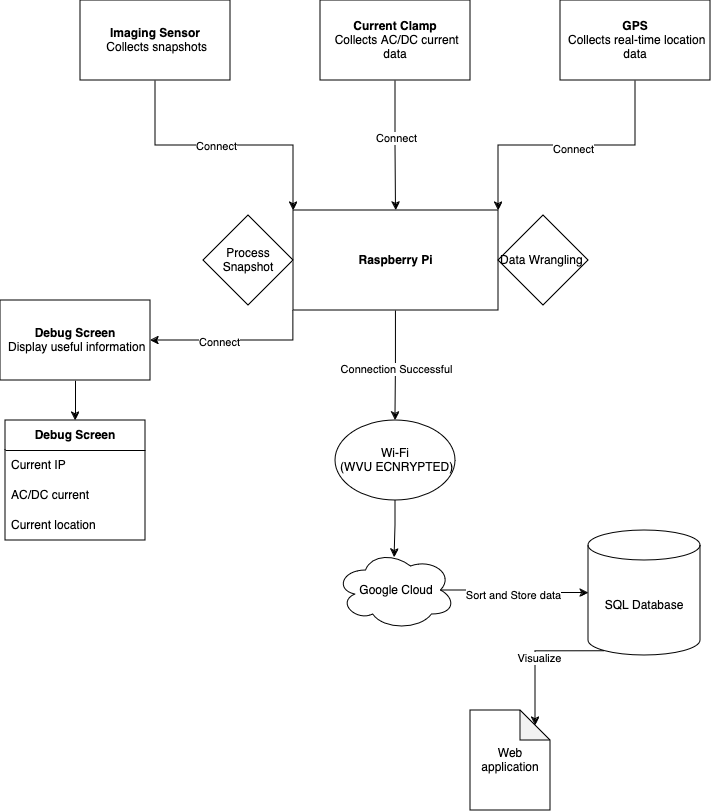
\includegraphics[width=0.5\textwidth]{System_Functionality.png}\\
    Fig 3. System Functionality
\end{center}

\subsubsection{Hardware}
Four devices fit onto the Raspberry Pi for the collection of data. 
The connections are shown below in Figure 4. 
The Pi communicates with the GPS for real-time location. 
The antenna plugs into the GPS and realizes the data collection. 
The current clamp collects AC voltage and current readings, recording it to the Pi.
A debug screen displays the GPS status, IP address, and the current AC reading for debugging purposes. 
The debug screen configures the subsystem, ensuring that the components work. 
Lastly, the imaging sensor collects snapshots of people for detecting the number of people in a PRT car. 
The snapshots go to the Raspberry Pi, where the Pi will use an algorithm to count the number of people in that snapshot.

\begin{center}
    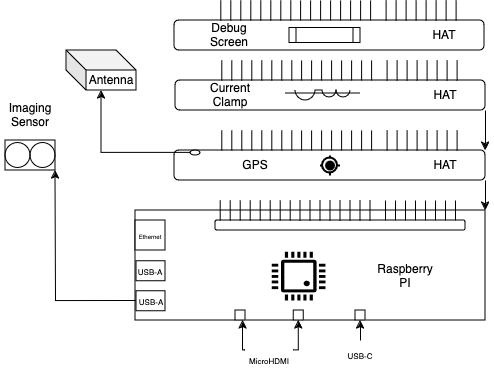
\includegraphics[width=0.5\textwidth]{Hardware_Architecture.png}\\
    Fig 4. Hardware Architecture
\end{center}

\subsubsection{Software}
When the Raspberry Pi obtains a Wi-Fi connection through WVU Encrypted and is at a standstill for 5 seconds or more, data goes to Google Cloud. 
Figure 5 represents the process of data transfer once Wi-Fi connects. 
The Google Cloud hosts a SQL database that sorts and stores all the metadata from the Pi system. 
A web application uses this sorted data from the SQL database, providing visualization through charts and graphs to highlight relationships in the data. 
The web application provides opportunities for identifying potential risks in the system, such as irregular AC current or voltage on a specific PRT car.

\begin{center}
    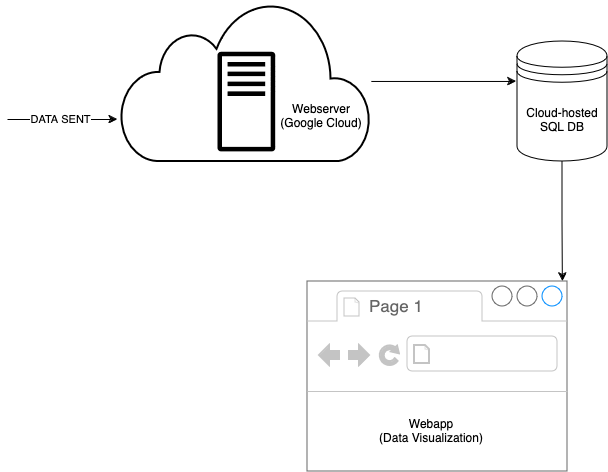
\includegraphics[width=0.5\textwidth]{Software_Architecture.png}\\
    Fig 5. Software Architecture
\end{center}

\subsection{System Design}
\subsection{Overall Architecture}
\input{sections/system design/overall architecture.tex}

\subsection{System Design}
\input{sections/system design/system design.tex}

\subsection{Risks}

\subsection{Test Plans}
\subparagraph{GPS Data Visualization Proof of Concept:}
\subparagraph{Current Clamp Testing with Space Heater:}

\subsection{Risks}

\subsection{Test Plans}
\subparagraph{GPS Data Visualization Proof of Concept:}
\subparagraph{Current Clamp Testing with Space Heater:}

\subsection{Risks}

\subsection{Test Plans}
\subparagraph{GPS Data Visualization Proof of Concept:}
\subparagraph{Current Clamp Testing with Space Heater:}

\subsection{Risks}
As with any project, there are risks involved in implementation of this project. 
For the PRT cars, environmental factors like rainy weather conditions or elevated heat or cold temperatures may pose a threat to the data collection system or impact the system performance.

In order for the project to be a convenient solution for the data collection problem, the solution needs to be easily maintainable. 
Ensuring maintainability is crucial post-installation for system accessibility. 

Security is paramount, with data encryption and secure transmission protocols mitigating risks. 

Additionally, the choice of LiDAR sensors directly affects passenger eye health, highlighting the importance of careful selection.


\subsection{Test Plans}
To ensure that our solution meets the requirements specified, multiple stages and techniques of testing will be conducted. 
As we are currently developing proofs of concept, our testing for this stage involves gathering data and observing that it is accurate and useful. 
It is during this stage that we must observe the practicality of our initial ideas, noting what works and what doesn’t.

Once the proof of concept for the entire design can be established, the next stage of testing will involve implementing a fully functional prototype in an environment that resembles the goal environment. 
For this project, that environment is the PRT. 
We must simulate the PRT, to the best of our ability, to create a demonstration of the product. 
In this environment we will observe how our solution performs, measuring it against our predetermined goals. 

Then, the solution must be stress tested to determine how the system will perform under different circumstances, some being situations that are not ideal. 
By doing this, we can properly communicate the ranges of which the solution works.

Once determined that the implementation is ready for use on the PRT, the data collection will begin on just a single car. 
Should the system perform to standards, it could then be implemented on all cars in the PRT System.

\subparagraph{GPS Data Visualization Proof of Concept:}
\textit{Objective:} Using the GPS on the PRT to visualize a path as proof of concept.

\textit{Procedure:} We will be attaching the GPS to the PRT vehicle and record its path through the GPS data. We will then use the test run to help us visualize the path traveled by the PRT vehicle.

\textit{Outcome to be achieved:} We should be able to visualize the route from the GPS data and this will then demonstrate the effectiveness of the data collected by the GPS data during its route.

\subparagraph{Current Clamp Testing with Space Heater:}
\textit{Objective:} Verify the functionality of the current clamp on a space heater to show its effectiveness as a subtitle for the internal PRT

\textit{Procedure:} We will attach the current clamp to a space heater and record its power usage. We will take and analyze the data received from this and measure the power of consumption.

\textit{Outcome to be achieved:} We should be able to retrieve data from the space heater that shows the current clamp is accurate and working perfectly.
